\documentclass[border=10pt]{standalone}
\usepackage{ifthen}
\usepackage{tikz}
\usetikzlibrary{
  arrows,
  arrows.meta,
}
\usepackage{pgfplots}
\usepgfplotslibrary{
    fillbetween,
}
\usetikzlibrary[calc]

\begin{document}

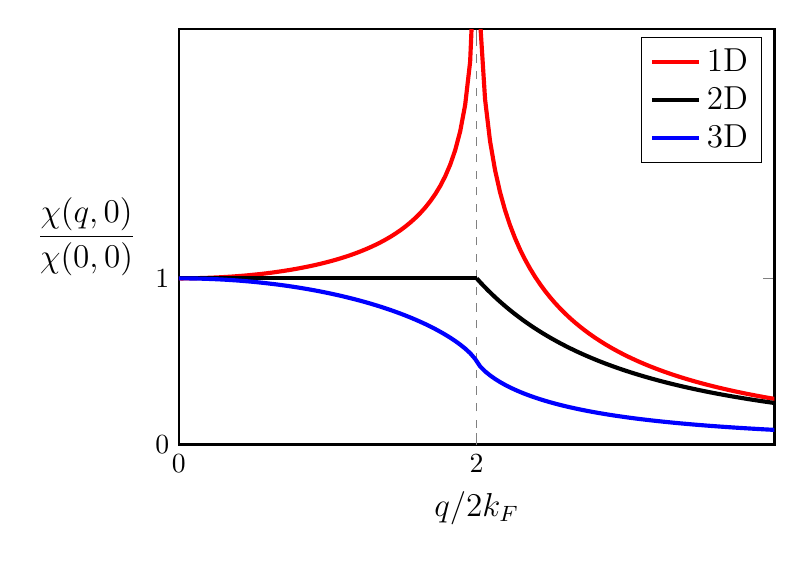
\begin{tikzpicture}
  \begin{axis}
    [
        declare function = {
          lindhard1(\t) = (1 / \t) * ln(abs((\t + 2)/(\t - 2)));
          lindhard2(\t) = 4 / (\t^2);
          lindhard3(\t) = (1 / 2) * (1 - 0.25*\t*(1 - 4/(\t^2))*ln(abs((\t + 2)/(\t - 2))));
        },
        width=3.6in, height=2.7in,
        xmin=0, xmax=4,
        ymin=0, ymax=2.5,
        legend entries = {1D, 2D, 3D},
        legend style = {font=\large},
        xlabel = {$q / 2k_F$},
        ylabel = {$\displaystyle\frac{\chi(q, 0)}{\chi(0, 0)}$},
        xlabel style= {font=\large},
        ylabel style= {rotate=-90, font=\large},
        xtick={0, 2},
        ytick={0, 1},
        axis line style = {line width=1.0pt},
    ]
    % q = 2 k_F
    \addplot[forget plot, dashed, line width=0.5pt, color=gray] coordinates {(2, 0) (2, 4)};
    
    % Lindhard response function for 1D electron gas
    \addplot[samples=300, color=red, line width=1.5pt] {lindhard1(x)};
    
    % do not show legend for this plot: "forget plot"
    \addplot[samples=10, domain=0:2, color=black, line width=1.5pt, forget plot] {1};
    % Lindhard response function for 2D electron gas
    \addplot[samples=300, domain=2:4, color=black, line width=1.5pt] {lindhard2(x)};

    % Lindhard response function for 3D electron gas
    \addplot[samples=300, color=blue, line width=1.5pt] {lindhard3(x)};
  \end{axis}
\end{tikzpicture}

\end{document}
